\documentclass{beamer}
\usepackage{beamerthemesplit}
% \usepackage{pstricks}
\usepackage{graphicx}
\usepackage{mdwlist}
\usepackage{lineno, hyperref}

\usepackage{amssymb,latexsym,amsmath,amsthm,bbm}
\usepackage{hyperref}
\usepackage{tikz}
\usepackage[english]{babel}
\usepackage[latin1]{inputenc}
\usepackage{multirow}
\usepackage{verbatim}
\usepackage{alltt}
\usepackage{mycommands}

\usepackage{cmbright}
\renewcommand*\familydefault{\sfdefault}
\usepackage[T1]{fontenc}


\definecolor{wp-red}{RGB}{204,0,0}
\definecolor{wp-gray}{RGB}{51,51,51}
\definecolor{reynolds-red}{RGB}{153,0,0}
\definecolor{pyroman-flame}{RGB}{209,81,34}
\definecolor{hunt-yellow}{RGB}{253,215,38}
\definecolor{genomic-green}{RGB}{125,140,31}
\definecolor{innovation-blue}{RGB}{66,126,147}
\definecolor{bio-indigo}{RGB}{65,86,161}

\setbeamercolor{structure}{fg=wp-red}
\setbeamercolor{title}{bg=white, fg=wp-red}  % changes color on title page
\setbeamerfont{title}{series=\bfseries, size=\huge}
\setbeamerfont{author}{series=\bfseries, size=\Large}
\setbeamerfont{institute}{series=\mdseries, size=\large}

\setbeamercolor{frametitle}{bg=wp-red, fg=white}  % changes color at top of frame
\setbeamerfont{frametitle}{series=\bfseries}
\setbeamercolor{title in head/foot}{fg=white, bg=wp-red}  % changes color for title in footer
\setbeamerfont{title in head/foot}{series=\bfseries}
\setbeamercolor{author in head/foot}{fg=white,bg=wp-gray}  % changes color for author in footer
\setbeamerfont{author in head/foot}{series=\bfseries}


\title[Spatiotemporal Modeling of Extreme Events] % (optional, use only with long paper titles)
{
  Spatiotemporal Modeling of Extreme Events
}
\author[S. Morris and B. Reich]{Samuel Morris and Brian Reich}
\institute[NCSU]{North Carolina State University}
\date{}

\begin{document}

\begin{frame}\frametitle{\ }
\begin{center}
	\maketitle
\end{center}
\end{frame}

\begin{frame}{Motivation}
  \begin{itemize} \setlength{\itemsep}{1em}
    \item Average behavior is important to understand, but it does not paint the whole picture.
    \begin{itemize}
      \item e.g. When constructing river levees, engineers need to be able to estimate a 100-year or 1000-year flood levels.
    \end{itemize}
    \item In geostatistical analysis, kriging uses spatial correlation to help inform prediction at unknown locations.
    \item Want to explore computationally easy methods that are available in higher dimensions
  \end{itemize}
\end{frame}

% \begin{frame}{Introduction to extremes}
%   \begin{itemize} \setlength{\itemsep}{0.5em}
%     \item Max-stable processes (Cooley et al., 2012):
%     \begin{itemize}
%       \item Consider a spatial process $x_t(\bs)$, $t = 1, \ldots, T$.
%       \item Let $M_T(\bs) = \left\{ \bigvee_{t=1}^T x_t(\bs_1), \ldots, \bigvee_{t=1}^T x_t(\bs_n) \right\}$
%       \item If there exists normalizing sequences $a_T(\bs)$ and $b_T(\bs)$ such
%       that for all sites, $\bs_i, i = 1, \ldots, d$,
%       \begin{align*}
%         a_T^{-1}(\bs) \left\{ M_T(\bs) - b_T(\bs) \right\} \converged Y(\bs)
%       \end{align*}
%       which has a non-degenerate distribution, then $Y(\bs)$ is a max-stable process.
%     \end{itemize}
%   \end{itemize}
% \end{frame}

\begin{frame}{Standard non-spatial analysis}
  \begin{itemize} \setlength{\itemsep}{0.5em}
    \item Block maxima:
    \begin{itemize}
      \item Uses yearly maxima
      \item Discards many observations
      \item Models are fit using the generalized extreme value distribution
    \end{itemize}
    \item Generalized extreme value distribution (GEV):
    \begin{align*}
      \Pr(Y_j < y) = G_j(y) = \exp \left\{ -\left[ \left(1 + \xi_j \frac{y - \mu_j}{\sigma_j}\right)_+^{-1/\xi_j} \right] \right\}
    \end{align*}
  \end{itemize}
\end{frame}

\begin{frame}{Standard non-spatial analysis}
  \begin{itemize}
    \item Peaks-over-threshold:
    \begin{itemize}
      \item Incorporates more data than block maxima
      \item Select a threshold, $T$, and fit data above the threshold using the generalized Pareto distribution
      \item Autocorrelation may be an issue between observations (e.g. flood levels don't dissipate overnight)
    \end{itemize}
    \item Generalized Pareto distribution (GPD):
    \begin{align*}
      \Pr(Y_j > y | Y_j > T) = F_j(y) = \left( 1 + \xi_j \frac{y - T}{\sigma_j} \right)_+^{-1/\xi_j}
    \end{align*}
  \end{itemize}
\end{frame}

% \begin{frame}{Multivariate representations}
%   \begin{itemize}
%     \item Multivariate distributions:
%     \begin{itemize}
%       \item Assume common standardized max-stable marginal, like unit-Fr\'{e}chet
%       \begin{align*}
%         \Pr(Z < z) = exp(-z^{-1})
%       \end{align*}
%       \item The multivariate representation for the GEV is
%       \begin{align*}
%         \Pr(\bZ \le \bz)  &= G^*(\bz) = \exp(-V(\bz))\\
%                 V(\bs)    &= d \int_{\Delta_d} \bigvee_{i = 1}^d \frac{w_i}{z_i} H(\ddd w)
%       \end{align*}
%       where
%       \begin{itemize}
%         \item $\Delta_d = \{ \bw \in \calR^d_+ \mid w_1 + \cdots + w_d = 1\}$
%         \item $H$ is a probability measure on $\Delta_d$
%         \item $\int_{\Delta_d}w_i H(\ddd w) = 1 / d$ for $i = 1, \ldots, d$.
%       \end{itemize}
%     \end{itemize}
%   \end{itemize}
% \end{frame}

\begin{frame}{Multivariate analysis}
  \begin{itemize} \setlength{\itemsep}{0.5em}
    \item Multivariate max-stable and GPD models have nice features, but they are
    \begin{itemize}
      \item computationally hard to work with
      \item joint distribution only available in low dimension
    \end{itemize}
    \item Pairwise likelihood approach (Huser and Davison, 2014)
  \end{itemize}
\end{frame}

\begin{frame}{Model objectives}
  \begin{itemize} \setlength{\itemsep}{0.5em}
    \item Our objective is to build a model that
    \begin{itemize}
      \item has a flexible tail
      \item has asymptotic spatial dependence
      \item computation on the order of Gaussian models for large space-time datasets
    \end{itemize}
  \end{itemize}
\end{frame}

\begin{frame}{Thresholding data}
  \begin{itemize} \setlength{\itemsep}{0.5em}
    \item We threshold the observed data at a high threshold $T$.
    \item Thresholded data:
    \begin{align*}
      Y_t^*(\bs) = \left\{ \begin{array}{ll}
          Y_t(\bs) \quad & Y_t(\bs) > T\\
          T \quad & Y_t(\bs) \le T
      \end{array}\right.
    \end{align*}
    \item Allows tails of the distribution to speak for themselves.
  \end{itemize}
\end{frame}

\begin{frame}{Spatial skew-$t$ distribution}
  \begin{itemize} \setlength{\itemsep}{0.5em}
    \item Assume observed data $Y_t(\bs)$ come from a skew-$t$ (Zhang and El-Shaarawi, 2012)
    \begin{align*}
      Y_t(\bs) = X_t(\bs)\beta + \alpha z_t + v_t(\bs)
    \end{align*}
    where
    \begin{itemize} \setlength{\itemsep}{0.25em}
      \item $\alpha \in \calR$ controls the skew
      \item $z_t \iid N_{(0, \infty)}(0, \sigma^2_t)$ is a random effect
      \item $v_t(\bs)$ is a Gaussian process with variance $\sigma^2_t$ and \Matern correlation
      \item $\sigma_t^2 \iid \text{IG}(a, b)$
    \end{itemize}
  \end{itemize}
\end{frame}

\begin{frame}{Skew-normal distribution}
  \begin{itemize} \setlength{\itemsep}{0.5em}
    \item Conditioned on $z_t$ and $\sigma^2_t$, $Y_t(\bs)$ is Gaussian
    \begin{itemize}
      \item After marginalizing over $\sigma^2_t$, this becomes a multivariate $t$-distribution with $2a$ degrees of freedom.
    \end{itemize}
    \item Can use standard geostatistical methods to fit this model.
    \item Predictions can be made through kriging.
    \item Marginalizing over $z_t$ and $\sigma^2_t$ (via MCMC),
    \begin{align*}
      Y_t(\bs) \sim \text{skew-t}(\mu, \alpha, \text{df}=2a)
    \end{align*}
  \end{itemize}
\end{frame}

\begin{frame}{Long-range dependence}
  \begin{itemize} \setlength{\itemsep}{0.5em}
    \item The $\chi$ coefficient is a measure of extremal spatial correlation
    \begin{align*}
      \chi(\bh) = \Pr(Y_t(\bs) > c \mid Y_t(\bs + \bh) > c)
    \end{align*}
    \item This value shows asymptotic dependence that does not approach 0 as $\bh \rightarrow \infty$.
    \item Deal with this through a daily random partition.
  \end{itemize}
\end{frame}

\begin{frame}{Random daily partition}
  \begin{itemize} \setlength{\itemsep}{0.5em}
    \item Daily random partition allows $z_t$ and $\sigma^2_t$ to vary by site.
    \begin{align*}
      Y_t(\bs) = X_t(\bs) \beta + \alpha z_t(\bs) + v_t(\bs)
    \end{align*}
    \item Consider a set of daily knots $\{w_{t1}, \ldots, w_{tK}\}$ that define a daily partition
    $\{P_{t1}, \ldots, P_{tK}\}$ such that
    \begin{align*}
      P_{tk} = \{s : k = \argmin_\ell|| \bs - w_{t\ell}|| \}
    \end{align*}
    \item For $\bs \in P_{tk}$
    \begin{align*}
      z_t(\bs) &= z_{tk}\\
      \sigma^2_t(\bs) &= \sigma^2_{tk}
    \end{align*}
    \item Within each partition $Y_t(\bs)$ has the same distribution as before.
  \end{itemize}
\end{frame}


\begin{frame}{MCMC details}
  \begin{itemize} \setlength{\itemsep}{0.5em}
    \item Three main steps:
    \begin{enumerate}[1.]
      \item Impute missing observations and data below $T$
      \item Update parameters with random walk Metropolis Hastings or Gibbs sampling
      \item Make spatial predictions
    \end{enumerate}
    \item Priors are selected to be conjugate when possible.
  \end{itemize}
\end{frame}

\begin{frame}{Data analysis}
  \begin{itemize} \setlength{\itemsep}{0.5em}
    \item Ozone analysis at 85 sites in NC, SC, and GA for 92 days
    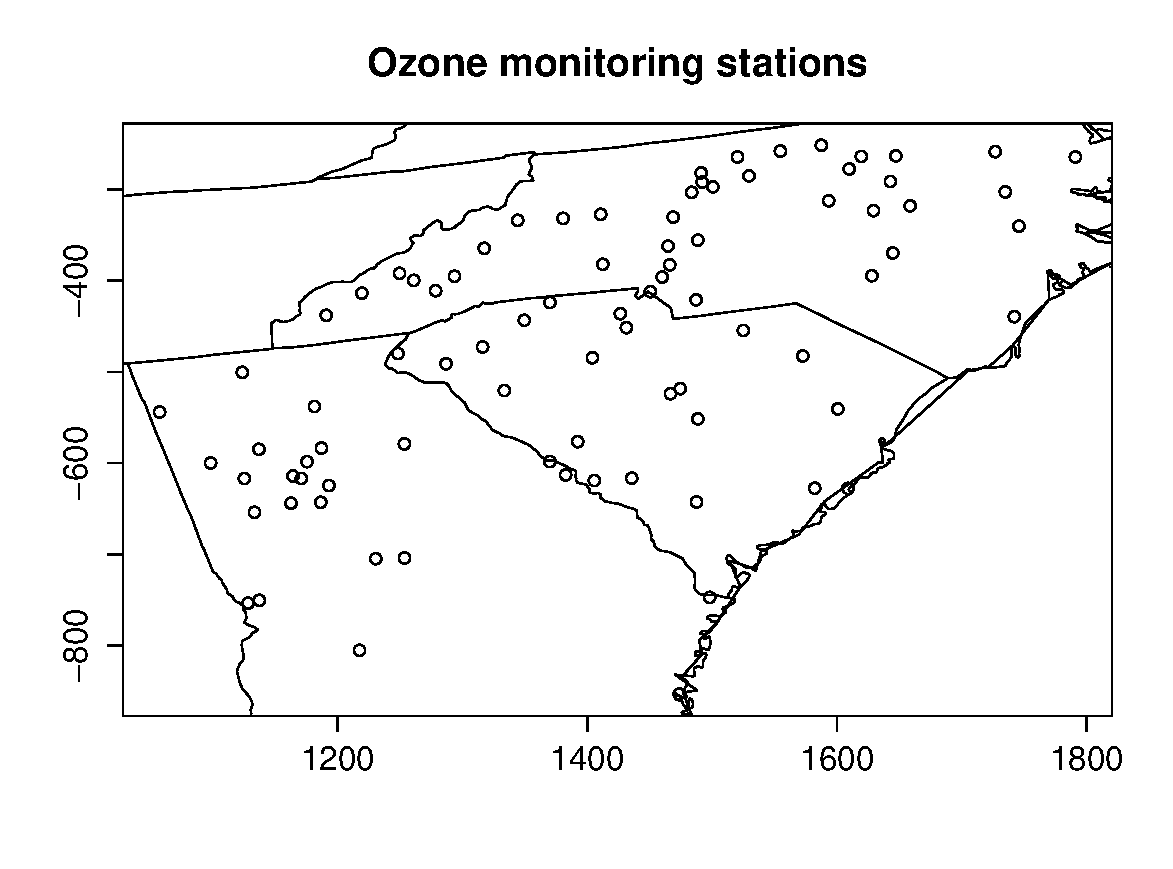
\includegraphics[width=1\linewidth]{./plots/ozone_station.pdf}
  \end{itemize}
\end{frame}

\begin{frame}{Model comparisons}
  \begin{itemize} \setlength{\itemsep}{0.5em}
    \item 9 different analysis methods incorporating
    \begin{itemize}
      \item Gaussian vs $t$
      \item 1 partition vs 5 partitions
      \item No thresholding vs thresholded
      \begin{itemize}
        \item Thresholded data at 0.90 sample quantile
      \end{itemize}
    \end{itemize}
    \item All methods use a \Matern or exponential covariance ($\nu = 0.5$)
    \item Compare quantile and Brier scores using 5-fold cross validation
    \item Mean function modeled using a first-order spatial trend
  \end{itemize}
\end{frame}

\begin{frame}{Cross-validation results}
  \begin{table}[htbp]
    \small
    \centering
    \begin{tabular}{lrrrrrr}
           & \multicolumn{6}{c}{Quantile}\\
           \cline{2-7}
    & 0.900 & 0.950 & 0.980 & 0.990 & 0.995 & 0.999\\
  \hline
Gaussian & 16.38 & 15.76 & 15.02 & 14.52 & 14.08 & 13.22\\
$t$-1 ($T=0$) & 16.15 & 15.51 & 14.62 & 14.00 & 13.43 & 12.32\\
$t$-5 ($T=0$) & 13.61 & 12.66 & 11.61 & 10.96 & 10.40 & 9.34\\
$t$-1 ($T=0.9$) & 5.52  & 3.58  & 2.28  & 1.77  & 1.47  & 1.10\\
$t$-5 ($T=0.9$) & 5.98  & 4.27  & 2.99  & 2.41  & 2.03  & 1.49\\
skew $t$-1 ($T=0$) & 9.24  & 7.27  & 5.26  & 4.13  & 3.27  & 1.96\\
skew $t$-1 ($T=0.9$) & {\bf 4.91}  & {\bf 3.16} & {\bf 1.94}  & {\bf 1.45}  & {\bf 1.16}  & {\bf 0.82}\\
skew $t$-5 ($T=0$) & 15.81 & 14.46 & 12.74 & 11.57 & 10.57 & 8.60\\
skew $t$-5 ($T=0.9$) & & & & & &\\
\hline
    \end{tabular}
  \end{table}
  \begin{itemize} \setlength{\itemsep}{0.5em}
    \item Quantile scores -- Still waiting on last set
  \end{itemize}
\end{frame}

\begin{frame}{Simulation study settings}
  \begin{itemize} \setlength{\itemsep}{0.5em}
    \item Data generated from 6 different settings.
    \begin{enumerate}[1.]
      \item Gaussian
      \item $t$-1 with 4 degrees of freedom
      \item $t$-5 with 4 degrees of freedom
      \item skew $t$-1 with 4 degrees of freedom ($\alpha = 3$)
      \item skew $t$-5 with 4 degrees of freedom ($\alpha = 3$)
      \item Half-Gaussian, Half $t$-1 (spatial range = 0.4)
    \end{enumerate}
    \item Spatial settings
    \begin{itemize}
      \item $\bs \in [0, 1] \times [0, 1]$
      \item Exponential covariance with range: 0.1
      \item Ratio of spatial to nugget error: 0.9
    \end{itemize}
  \end{itemize}
\end{frame}

\begin{frame}{Simulation study methods}
  \begin{itemize} \setlength{\itemsep}{0.5em}
    \item 5 different analysis methods
    \begin{enumerate}[1.]
      \item Gaussian
      \item Skew $t$-1 ($T=0$)
      \item Skew $t$-1 ($T=0.9$)
      \item Skew $t$-5 ($T=0$)
      \item Skew $t$-5 ($T=0.9$)
    \end{enumerate}
    \item All methods use a \Matern covariance structure except for method 5 which uses an exponential covariance ($\nu = 0.5$)
  \end{itemize}
\end{frame}

\begin{frame}{Simulation results}
  Still rerunning a few of the MCMC runs because quantile scores for 4. and 5. are
  unusually high for method 5
\end{frame}

\begin{frame}{Future work}
  \begin{itemize} \setlength{\itemsep}{0.5em}
    \item Comparison with extreme value analysis methods
    \item Including time in the model
    \begin{itemize}
      \item AR(1): $Y_t(\bs) = X_t(\bs) \beta + \phi Y_{t-1}(\bs) + \alpha z_t(\bs) + v_t(\bs)$
    \end{itemize}
  \end{itemize}
\end{frame}

\begin{frame}{Questions}
  \begin{itemize} \setlength{\itemsep}{0.5em}
    \item Any questions?
    \item Thank you for your attention.
  \end{itemize}
\end{frame}

\begin{frame}{References}
  \begin{itemize} \setlength{\itemsep}{0.5em}
    \item Cooley, D., Cisewski, J., Erhardt, R. J., Mannshardt, E., Omolo, B. O. and Sun, Y. (2012) A survey of spatial extremes: Measuring spatial dependence and modeling spatial effects. {\it REVSTAT}, {\bf 10}, 135--165.
    \item Huser, R. and Davison, A. C. (2014) Space-time modelling of extreme events. {\it Journal of the Royal Statistical Society: Series B (Statistical Methodology)}, {\bf 76}, 439--461
    \item Zhang, H. and El-Shaarawi, A. (2010) On spatial skew-Gaussian processes and applications. {\it Environmetrics}, {\bf 21} 33--47.
  \end{itemize}
\end{frame}

\end{document}